%
%
% SUMMARY:
% USAGE:
%
% AUTHOR:       Gilles Fourestey
% ORG:          EPFL
% E-MAIL:       foureste@iacspc.epfl.ch
%
% ORIG-DATE: 21-Nov-08 at 11:16:22
% LAST-MOD: 10-Feb-09 at 14:19:48 by Gilles Fourestey
%
% DESCRIPTION:
% DESCRIP-END.


\chapter{Learning by examples}
\label{cha:examples}


\section{Reading data}
\label{sec:readingData}
In order to read input data, LifeV is integrated with the open-source library \verb!GetPot! (\url{http://getpot.sourceforge.net/}). GetPot allows to easily handle the data regarding the different phases of the simulation, typically providing the mesh name, the discretization order, the physical parameters, the solver information and the time step (if any).
\newline
\noindent \verb!GetPot! needs the name of the input file that can be linked through the flags "-f" or "--file" while launching the
program, e.g. 
\begin{lstlisting}
$ ./myProgram.exe -f myData
\end{lstlisting}
The GetPot object allows to read the data from the file, and is constructed thanks to the name of the input file. 
If no name is provided, then LifeV uses the default input name "data".
\begin{lstlisting}
GetPot command_line(argc,argv);
const std::string dataFileName = command_line.follow("data", 2, "-f","--file");
GetPot dataFile(dataFileName);
\end{lstlisting}
\noindent
The input file must have a tree-structure, an example is as follows
\begin{lstlisting}
# -*- getpot -*- (GetPot mode activation for emacs)
#-------------------------------------------------
#      Data file for the Laplacian example
#-------------------------------------------------

[finite_element]
    degree                       = P1

[mesh]
    nx                           = 40
    ny                           = 40
    nz                           = 40
    overlap                      = 0
    verbose                      = false

[prec]
    prectype                     = Ifpack # Ifpack or ML
    displayList                  = false

    [./ifpack]
        overlap                  = 2

        [./fact]
            ilut_level-of-fill   = 1
            drop_tolerance       = 1.e-5
            relax_value          = 100

    [../amesos]
        solvertype               = Amesos_KLU #Amesos_KLU or Amesos_Umfpack

    [../partitioner]
        overlap                  = 0

    [../schwarz]
        reordering_type          = none #metis, rcm, none
        filter_singletons        = true

    [../]
[../]
\end{lstlisting}
\noindent
and the data can be read as in folders. For instance, if we have the previous data file and we want to print the mesh sizes in the three directions,
we only need to type

\begin{lstlisting}
std::cout << "Number of elements in each direction" 
          << "x: " dataFile( "mesh/nx", 15 )
          << "y: " dataFile( "mesh/ny", 15 )
          << "z: " dataFile( "mesh/nz", 15 )
          << std::endl;
\end{lstlisting}
\noindent
where the values "15" are set in LifeV as default sizes. More generally, in every LifeV-based program, we need to access in the same manner the data through the GetPot object, providing also a safe default value in case some variables are not specifically set.

\noindent
You can browse the default data file in every testsuite directory to see examples. Generally, some entries are compulsory (e.g. the mesh name for unstructured meshes), on the other hand others are filled with a default value if not specified in the input file. \\






\section{The Poisson problem}
\label{sec:poisson}
In this section, we go through a first example dealing with the Poisson equation. At first we introduce the mathematical setting and well-posedness of the problem, presenting its finite dimensional formulation and the error estimates. Then we explain how to solve the Poisson problem using LifeV, going through the different stages that characterize the simulation. More in particular, we will cover the following topics: 
\begin{itemize}
	\item the preamble: including the headers and configuring MPI
	\item the construction of a structured mesh and the definition of the finite elements space
	\item the assembly of the stiffness matrix, the right-hand-side and the setting of boundary conditions
	\item the preconditioner and the solution of the linear system
	\item the exporting of data and the post-processing
\end{itemize}



\subsection{Variational formulation and finite element discretization}
Let $ \Omega \subset \mathbb{R}^d, \, d = 2,3 $ be a regular open bounded domain and let $  \partial \Omega $ be its boundary such that $ \partial \Omega = \Gamma_D \cup \Gamma_N$, $ \mathring{\Gamma}_D \cap \mathring{\Gamma}_N = \emptyset $, our problem reads

\begin{align}
\begin{cases}
\nonumber
-\Delta u = f \qquad & \mathbf{x} \in \Omega,
\\  \label{eq:poisson}
u = g(\mathbf{\sigma}) \qquad & \mathbf{\sigma} \in \Gamma_D,
\\ \nonumber
\partial_n u = h(\mathbf{\sigma}) \qquad & \mathbf{\sigma} \in \Gamma_N,
\end{cases}
\end{align}
\noindent
where $ f = f(\mathbf{x}) $ denotes the source term and $  g(\mathbf{\sigma}), h(\mathbf{\sigma}) $ denote the Dirichlet and Neumann boundary conditions, respectively. Starting from the differential equation, we can derive the weak formulation of the problem. We introduce the spaces
\begin{align}
	V &= H^1_d(\Omega) = \Bigl\{ v \in H^1(\Omega): v|_{\Gamma_D} = 0 \Bigr\}
\end{align}
and
\begin{align}
	V_g &= \Bigl\{ v \in H^1(\Omega): v|_{\Gamma_D} = g(\sigma) \Bigr\}.
\end{align}
Finally, our problem reads: find $ u \in V_g $, such that  
\begin{align}\label{eq:varPoisson}
a(u, v) = Fv \qquad \forall v \in V,
\end{align}
where
\begin{align} 
	a(u, v) = \int_{\Omega} \nabla u \cdot \nabla v d\mathbf{x} \qquad 
	\text{ and } \qquad 
	Fv = \int_{\Omega} f(\mathbf{x}) d\mathbf{x} + \int_{\Gamma_N} h(\sigma) d\sigma.
\end{align}
Under appropriate hypothesis, problem \eqref{eq:varPoisson} is well-posed.
In order to obtain a discrete solution of problem \eqref{eq:varPoisson} based on the finite element method, we introduce at first a partition $ \mathcal{T}_h $ of the domain $ \Omega $, and the finite-dimensional space
\begin{align}
V_h = X_h^r = \Bigl\{ v_h \in C^0(\bar{\Omega}): v_h|_K \in \mathbb{P}^r(), \forall K \in \mathcal{T}_h \Bigr\},
\end{align}
where $ \mathbb{P}^r $ denotes the polynomial functions of degree lower than or equal to $ r $. For sake of simplicity we suppose homogeneous Dirichlet boundary conditions, i.e. $ g = 0 $, in case $ g \neq 0 $, it is possible to operate a lifting to ring back to the homogeneous case. 
\newline \noindent
Finally, the finite dimensional problem reads: find $ u_h \in V_h $ such that 
\begin{align}\label{eq:fePoisson}
a(u_h, v_h) = Fv_h \qquad v_h \in V_h.
\end{align}
Starting from equation \eqref{eq:fePoisson}, it is possible to write the problems in the form of a linear system, and it is possible to prove that under appropriate assumptions about the data and the regularity of the exact solution $ u $, the discrete solution $ u_h $ satisfies the following error estimates
\begin{align}\label{eq:stimaHL}
& \|u-u_h\|_{L^2(\Omega)}  \leq Ch^{r+1}|u|_{H^{r+1}}, \\ &\nonumber \\ \label{eq:stimaH1}
& \|u-u_h\|_{H^1(\Omega)}  \leq Ch^r|u|_{H^{r+1}},
\end{align}
where $ h $ denotes the characteristic size of the mesh, $r$ the polynomial degree employed and $ C $ is a constant independent of $ h $ and $ u $, see e.g. \cite{CMCSBOOK2009002}.

\subsection{LifeV simulation}
To the aim of solving problem \eqref{eq:fePoisson} using LifeV, we set $ \Omega = (-1, 1)^3 $, $ \Gamma_D = \partial \Omega $ and the data $f, \, g, \, h $ such that the exact solution of the Poisson problem is  $ u(\mathbf{x}) = sin(\pi x)sin(\pi y)sin(\pi z) $.
\subsubsection*{Preamble: headers and MPI configuration}
We first include the different headers containing the data structures and the algorithms we are employing along the simulation: At first the Epetra data structures that allow the use of MPI
\begin{itemize}
\item the definition of the MPI environment, that is made exploiting the Epetra framework
\begin{lstlisting}
#include <Epetra_ConfigDefs.h>
#ifdef EPETRA_MPI
#include <mpi.h>
#include <Epetra_MpiComm.h>
#else
#include <Epetra_SerialComm.h>
#endif
\end{lstlisting}
\item the definition of the basis structures of LifeV, in particular meshes, finite elements spaces and expressions
\begin{lstlisting}
#include <lifev/core/LifeV.hpp>
#include <lifev/core/util/LifeChronoManager.hpp>
#include <lifev/core/mesh/MeshPartitioner.hpp>
#include <lifev/core/mesh/RegionMesh3DStructured.hpp>
#include <lifev/core/mesh/RegionMesh.hpp>
#include <lifev/core/array/MatrixEpetra.hpp>
#include <lifev/core/fem/BCManage.hpp>
#include <lifev/eta/fem/ETFESpace.hpp>
#include <lifev/eta/expression/BuildGraph.hpp>
#include <lifev/eta/expression/Integrate.hpp>
#include <Epetra_FECrsGraph.h>
\end{lstlisting}
\item the definition of the solver and the exporting routines
\begin{lstlisting}
#include <Teuchos_ParameterList.hpp>
#include <Teuchos_XMLParameterListHelpers.hpp>
#include <Teuchos_RCP.hpp>
#include <lifev/core/algorithm/LinearSolver.hpp>
#include <lifev/core/algorithm/PreconditionerIfpack.hpp>
#include <lifev/core/filter/ExporterHDF5.hpp>
\end{lstlisting}
\item some other useful classes
\begin{lstlisting}
#include <boost/shared_ptr.hpp>
#include <lifev/eta/examples/laplacian/laplacianFunctor.hpp>
\end{lstlisting}
Next, we define the LifeV namespace

\begin{lstlisting}
using namespace LifeV;


\end{lstlisting}

\subsubsection*{Structured mesh and finite element spaces}
After having read the datafile as explained in Section \ref{sec:readingData}, we build a cubic structured mesh and we divide it among the processors which are running the simulation

\begin{lstlisting}
// Mesh
typedef RegionMesh< LinearTetra > mesh_Type;
std::shared_ptr< mesh_Type > fullMeshPtr ( new mesh_Type ( Comm ) );
 
// Building structured mesh (in this case a cube)
regularMesh3D ( *fullMeshPtr, 0,
        dataFile( "mesh/nx", 15 ), dataFile( "mesh/ny", 15 ), 
        dataFile( "mesh/nz", 15 ), dataFile ( "mesh/verbose", false ),
        2.0, 2.0, 2.0, -1.0,-1.0, -1.0 );

// Partitioning mesh, possibly with overlap
const UInt overlap ( dataFile( "mesh/overlap", 0 ) );
std::shared_ptr< mesh_Type > localMeshPtr;

MeshPartitioner< mesh_Type > meshPart;

if ( overlap )
{
    meshPart.setPartitionOverlap ( overlap );
}
   
meshPart.doPartition ( fullMeshPtr, Comm );
localMeshPtr = meshPart.meshPartition();

// Clearing global mesh
fullMeshPtr.reset();
\end{lstlisting}    
We notice that the domain origins from the point $ (-1 -1, -1) $ and has a length of 2 in each dimension. The \verb!overlap! variable states the number of layers that are shared by two processors with contiguous subdomains.
\newline \noindent
We next define the finite element space, whose dimension is read by the input file. Then we build the corresponding Expression Template finite element space, whose use allows the user to adopt the templated expressions that refer to the weak formulation of the problem.
\begin{lstlisting}
// Finite element space
typedef FESpace< mesh_Type, MapEpetra >                 uSpaceStd_Type;
typedef std::shared_ptr< uSpaceStd_Type >             uSpaceStdPtr_Type;
typedef ETFESpace< mesh_Type, MapEpetra, 3, 1 >         uSpaceETA_Type;
typedef std::shared_ptr< uSpaceETA_Type >             uSpaceETAPtr_Type;
typedef FESpace<mesh_Type, MapEpetra>::function_Type    function_Type;

// Defining finite elements standard and Expression Template spaces
uSpaceStdPtr_Type uFESpace ( new uSpaceStd_Type ( localMeshPtr, 
                    dataFile( "finite_element/degree", "P1" ), 1, Comm ) );
uSpaceETAPtr_Type ETuFESpace ( new uSpaceETA_Type ( localMeshPtr, 
                    & ( uFESpace->refFE() ), & ( uFESpace->fe().geoMap() ), Comm ) );
\end{lstlisting}  

\subsubsection*{Assembly of the stiffness matrix, the right-hand-side and the setting of boundary conditions}
In order to assembly the system that corresponds to the finite element formulation, we need to build at first the graph that contains the topology of the matrix and then assemblying the matrix by constructing the elements $ a(\phi_j,\phi_i) $
\begin{lstlisting}
// Matrices and graphs
typedef Epetra_FECrsGraph                               graph_Type;
typedef std::shared_ptr<Epetra_FECrsGraph>            graphPtr_Type;
typedef MatrixEpetra< Real >                            matrix_Type;
typedef std::shared_ptr< MatrixEpetra< Real > >       matrixPtr_Type;

graphPtr_Type systemGraph;
matrixPtr_Type systemMatrix;

if ( overlap )
{
    systemGraph.reset ( new graph_Type ( Copy, * ( uFESpace->map().map( Unique ) ), 50, true ) );
}
else
{
    systemGraph.reset ( new graph_Type ( Copy, * ( uFESpace->map().map( Unique ) ), 50 ) );
}

{
    using namespace ExpressionAssembly;
    
    buildGraph (
            elements ( localMeshPtr ),
            uFESpace->qr(),
            ETuFESpace,
            ETuFESpace,
            dot ( grad ( phi_i ) , grad ( phi_j ) )
        )
        >> systemGraph;
}

systemGraph->GlobalAssemble();

if ( overlap )
{
systemMatrix.reset( new matrix_Type ( ETuFESpace->map(), *systemGraph, true ) );
}
else
{
systemMatrix.reset( new matrix_Type ( ETuFESpace->map(), *systemGraph ) );
}

// Clearing problem's matrix
systemMatrix->zero();

{
    using namespace ExpressionAssembly;
    
    integrate (
            elements ( localMeshPtr ),
            uFESpace->qr(),
            ETuFESpace,
            ETuFESpace,
            dot ( grad ( phi_i ) , grad ( phi_j ) )
        )
        >> systemMatrix;
}
\end{lstlisting}
Next, we build the solution and the right hand side vectors. For the latter, we employ the \verb!laplacianFunctor! class, that is constructed by providing the function that describes the source term
\begin{lstlisting}
// Vectors
typedef VectorEpetra                                    vector_Type;
typedef std::shared_ptr<VectorEpetra>                 vectorPtr_Type;

vectorPtr_Type rhsLap;
vectorPtr_Type solutionLap;

if ( overlap )
{
    rhsLap.reset ( new vector_Type ( uFESpace->map(), Unique, Zero ) );
    solutionLap.reset ( new vector_Type ( uFESpace->map(), Unique, Zero ) );
}
else
{
    rhsLap.reset ( new vector_Type ( uFESpace->map(), Unique ) );
    solutionLap.reset ( new vector_Type ( uFESpace->map(), Unique ) );
}

rhsLap->zero();
solutionLap->zero();

Real sourceFunction ( const Real& /*t*/, const Real& x, 
                      const Real& y, const Real& z, 
                      const ID& /*i*/)
{
    return 3 * M_PI * M_PI 
             * sin( M_PI * x )  * sin( M_PI * y ) * sin( M_PI * z );
}

std::shared_ptr<laplacianFunctor< Real > >  laplacianSourceFunctor ( new laplacianFunctor< Real >( sourceFunction ) );

{
    using namespace ExpressionAssembly;
    
    integrate (
            elements ( localMeshPtr ),
            uFESpace->qr(),
            ETuFESpace,
            eval(laplacianSourceFunctor, X) * phi_i
        )
        >> rhsLap;
}
\end{lstlisting}
We remark here that the use of the expression templates allows the user to define the equivalent of the weak formulation, in particular the elements of the matrix are built using the test and trial functions $ phi_i $ and $ phi_j $, and setting the quadrature rule to adopt.

\subsubsection*{Boundary conditions}
We explain here how to impose the boundary conditions. At first we give an identification number to the faces of our domain, and then define the function $ g $ that is assigned to the boundarues, in this case we have homogeneous Dirichlet conditions, so we construct the function \verb!zeroFunction! that returns 0. for every value of the spatial domain. In LifeV, it is possible to impose the boundaries through a BCHandler object, which imposes on every boundary the corresponding Dirichlet datum by providing the keyword \verb!Essential!.
\begin{lstlisting}
// Cube's walls identifiers
const int BACK   = 1;
const int FRONT  = 2;
const int LEFT   = 3;
const int RIGHT  = 4;
const int BOTTOM = 5;
const int TOP    = 6;

Real zeroFunction (const Real& /*t*/, const Real& /*x*/, const Real& /*y*/, const Real& /*z*/, const ID& /*i*/)
{
    return 0.;
}

BCHandler bcHandler;

BCFunctionBase ZeroBC ( zeroFunction );
BCFunctionBase OneBC ( nonZeroFunction );

bcHandler.addBC( "Back",   BACK,   Essential, Scalar, ZeroBC, 1 );
bcHandler.addBC( "Left",   LEFT,   Essential, Scalar, ZeroBC, 1 );
bcHandler.addBC( "Top",    TOP,    Essential, Scalar, ZeroBC, 1 );
bcHandler.addBC( "Front",  FRONT,  Essential, Scalar, ZeroBC, 1 );
bcHandler.addBC( "Right",  RIGHT,  Essential, Scalar, ZeroBC, 1 );
bcHandler.addBC( "Bottom", BOTTOM, Essential, Scalar, ZeroBC, 1 );

bcHandler.bcUpdate( *uFESpace->mesh(), uFESpace->feBd(), uFESpace->dof() );
bcManage ( *systemMatrix, *rhsLap, *uFESpace->mesh(), uFESpace->dof(), 
            bcHandler, uFESpace->feBd(), 1.0, 0.0 );
\end{lstlisting}

\subsubsection*{Preconditioning and solving the system}
Since our computation employs a parallel architecture. before solving the linear system we need to assemble both the matrix and the right hand side
\begin{lstlisting}
systemMatrix->globalAssemble();
rhsLap->globalAssemble();
\end{lstlisting}
Next we set the solver parameters according to the input file \verb!SolverParamList.xml! and the preconditioner that employs the Additive Schwarz method
\begin{lstlisting}
// Solver and preconditioner
typedef LinearSolver::SolverType                        solver_Type;
typedef LifeV::Preconditioner                           basePrec_Type;
typedef std::shared_ptr<basePrec_Type>                basePrecPtr_Type;
typedef PreconditionerIfpack                            prec_Type;
typedef std::shared_ptr<prec_Type>                    precPtr_Type;

LinearSolver linearSolver ( Comm );
linearSolver.setOperator ( systemMatrix );

Teuchos::RCP< Teuchos::ParameterList > aztecList = Teuchos::rcp ( new Teuchos::ParameterList );
aztecList = Teuchos::getParametersFromXmlFile ( "SolverParamList.xml" );

linearSolver.setParameters ( *aztecList );

prec_Type* precRawPtr;
basePrecPtr_Type precPtr;
precRawPtr = new prec_Type;
precRawPtr->setDataFromGetPot ( dataFile, "prec" );
precPtr.reset ( precRawPtr );

linearSolver.setPreconditioner ( precPtr );
\end{lstlisting}
And finally we solve the system
\begin{lstlisting}
linearSolver.setRightHandSide( rhsLap );
linearSolver.solve( solutionLap );
\end{lstlisting}



\subsubsection*{Exporting and post processing}
We set the exporter that employs the library HDF5, the result is then visible using a post processing tool, for instance Paraview (\url{http://www.paraview.org/}).
\begin{lstlisting}
// Setting exporter
ExporterHDF5< mesh_Type > exporter ( dataFile, "exporter" );
exporter.setMeshProcId( localMeshPtr, Comm->MyPID() );
exporter.setPrefix( "laplace" );
exporter.setPostDir( "./" );
exporter.addVariable ( ExporterData< mesh_Type >::ScalarField, "temperature", uFESpace, solutionLap, UInt ( 0 ) );
exporter.postProcess( 0 );
exporter.closeFile();
\end{lstlisting}

\begin{figure}
    \centering
    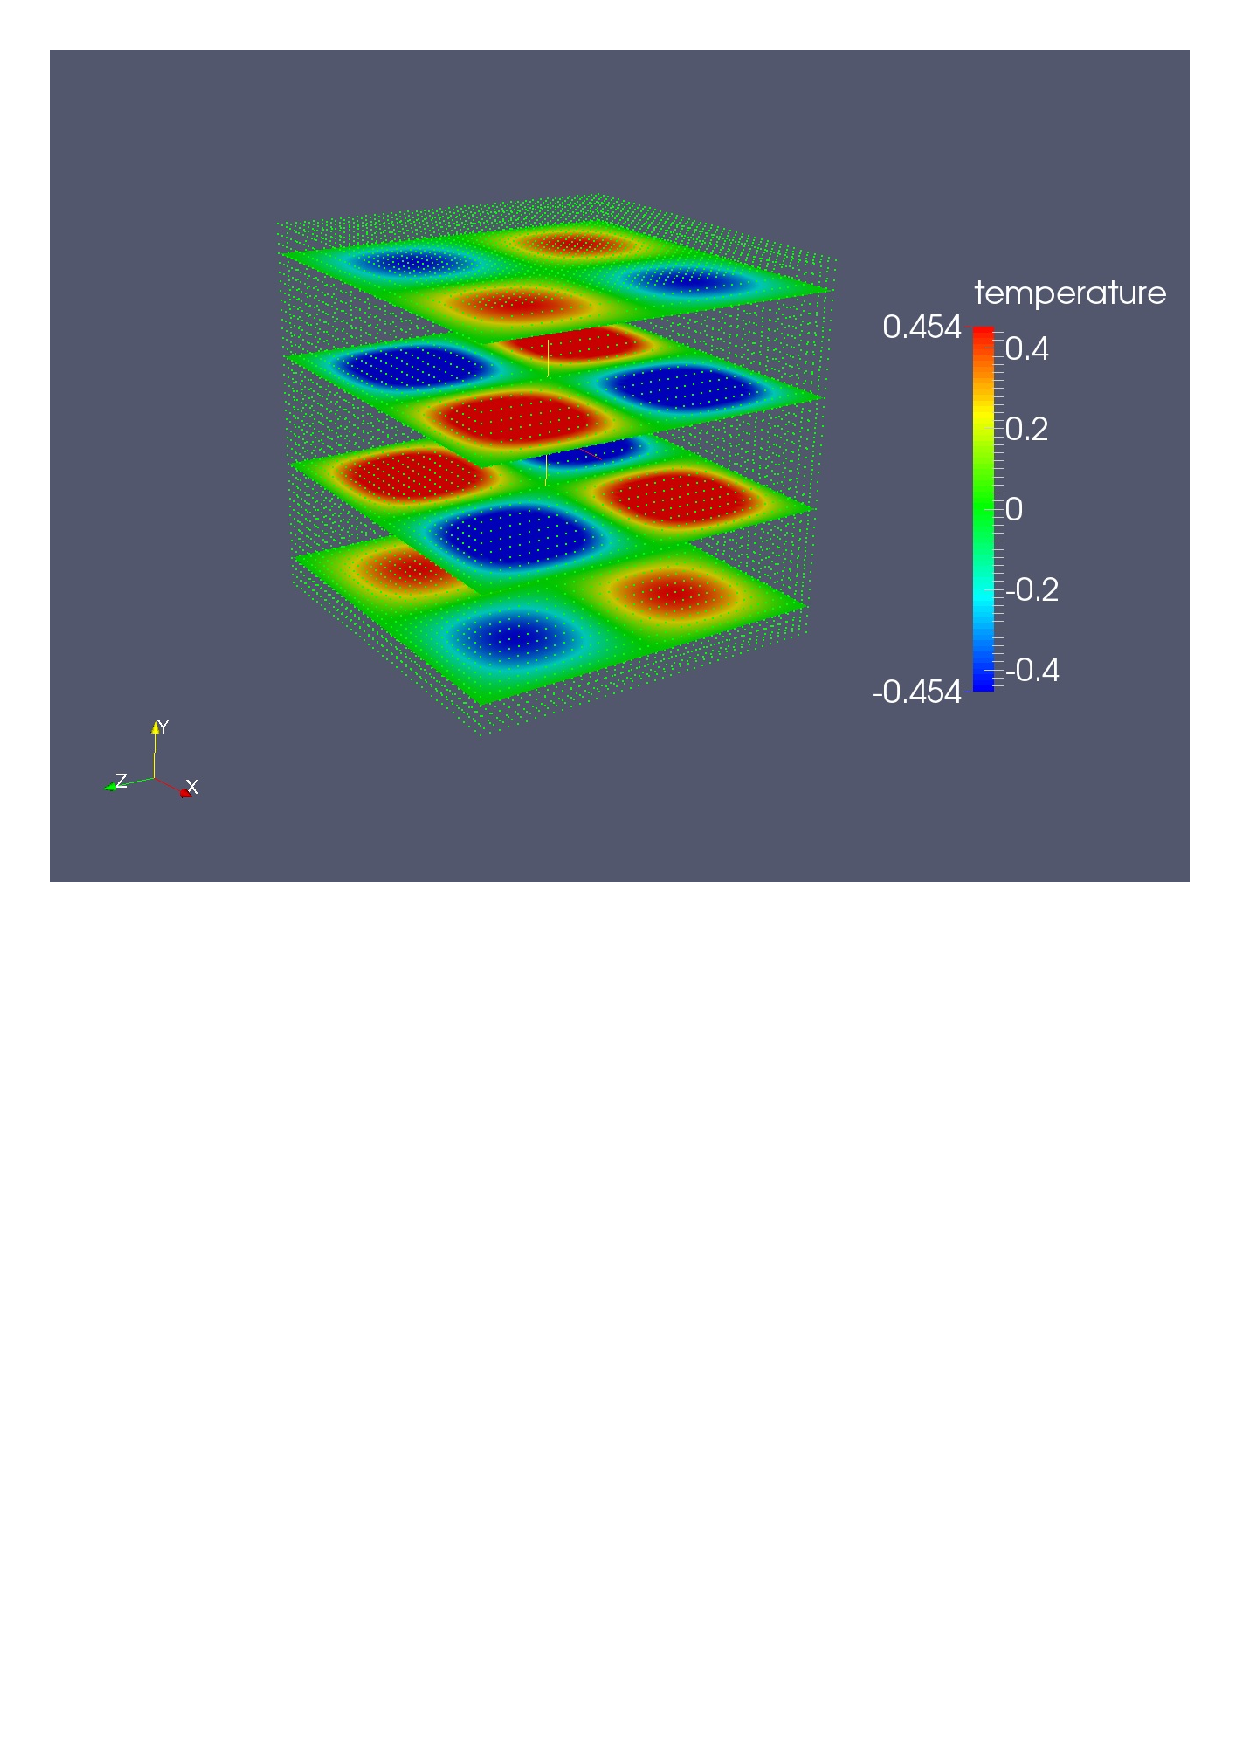
\includegraphics[width=\linewidth, trim=0cm 15cm 0cm 0cm, clip=true ]{pictures/slices}
    \caption{Result of Poisson equation with homogeneous Dirichlet boundary conditions}
    \label{fig:lap1}
\end{figure}
 
\newline \noindent
Now, suppose we want to investigate the trend of the error by varying the mesh size, to check numerically the estimates \eqref{eq:stimaHL}, \eqref{eq:stimaH1}. At first, we need to define the function $ u $ and its gradient $ \nabla u $ in our program, in the same way we defined the source term $f$
\begin{lstlisting}
Real uExactFunction (const Real& /*t*/, const Real& x, const Real& y, const Real& z, const ID& /*i*/)
{
    return sin( M_PI * y ) * sin( M_PI * z ) * sin ( M_PI * x );
}

function_Type uEx(uExactFunction);

VectorSmall< 3 > uGradExactFunction (const Real& /*t*/, const Real& x, const Real& y, const Real& z, const ID& /*i*/)
{
    VectorSmall< 3 > v;
    
    v[0] = M_PI * cos( M_PI * x ) * sin( M_PI * y ) * sin( M_PI * z );
    v[1] = M_PI * sin( M_PI * x ) * cos( M_PI * y ) * sin( M_PI * z );
    v[2] = M_PI * sin( M_PI * x ) * sin( M_PI * y ) * cos( M_PI * z );
    
    return v;
}

std::shared_ptr<laplacianFunctor< Real > >  laplacianExactFunctor ( new laplacianFunctor< Real >( uExactFunction ) );
std::shared_ptr<laplacianFunctor< VectorSmall<3> > >  laplacianExactGradientFunctor ( new laplacianFunctor< VectorSmall<3> >( uGradExactFunction ) );
\end{lstlisting}
Next, we need to evaluate the norms following their definition, and to do that we still employ the Expression Templates provided in LifeV
\begin{lstlisting}
Real L2ErrorLap = 0.0;
Real TotL2ErrorLap = 0.0;

Real H1SeminormLap = 0.0;
Real TotH1SeminormLap = 0.0;

{
    using namespace ExpressionAssembly;

    integrate (
            elements ( localMeshPtr ),
            uFESpace->qr(),
            ( eval(laplacianExactFunctor, X) - value (ETuFESpace, *solutionLap) )
            * ( eval(laplacianExactFunctor, X) - value (ETuFESpace, *solutionLap) )
        ) >> L2ErrorLap;

}

{
    using namespace ExpressionAssembly;
    
    integrate (
            elements ( localMeshPtr ),
            uFESpace->qr(),
            dot( eval(laplacianExactGradientFunctor, X) - grad( ETuFESpace, *solutionLap ),
            eval(laplacianExactGradientFunctor, X) - grad( ETuFESpace, *solutionLap ) )
        ) >> H1SeminormLap;
 
}
Comm->Barrier();
\end{lstlisting}
Finally, we gather the results of the different processors and print the norm. We collect the results for different mesh sizes and perform a convergence analysis, whose results are shown in Fig. \ref{fig:normHL}.
\begin{lstlisting}
Comm->SumAll (&L2ErrorLap, &TotL2ErrorLap, 1);
Comm->SumAll (&H1SeminormLap, &TotH1SeminormLap, 1);

if (verbose)
{
    std::cout << "TotError in L2 norm is " 
              << sqrt( TotL2ErrorLap ) << std::endl;
    std::cout << "TotError in H1 norm is " 
              << sqrt( TotL2ErrorLap + TotH1SeminormLap ) << std::endl;    
}
\end{lstlisting}

 
\begin{figure}
    \subfloat{
            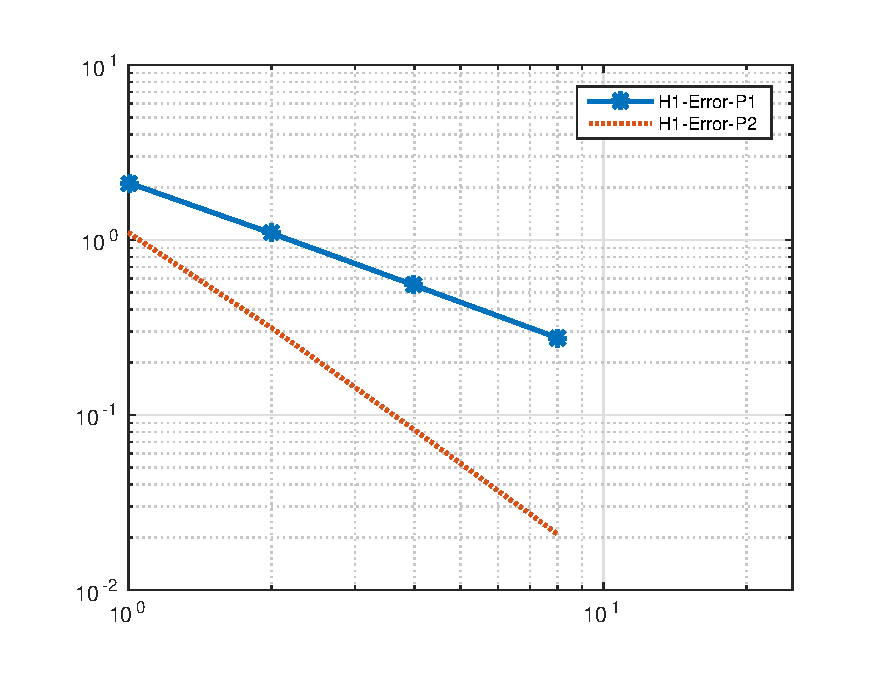
\includegraphics[width=.45\textwidth ]{pictures/convH1}
            }
    \subfloat{
            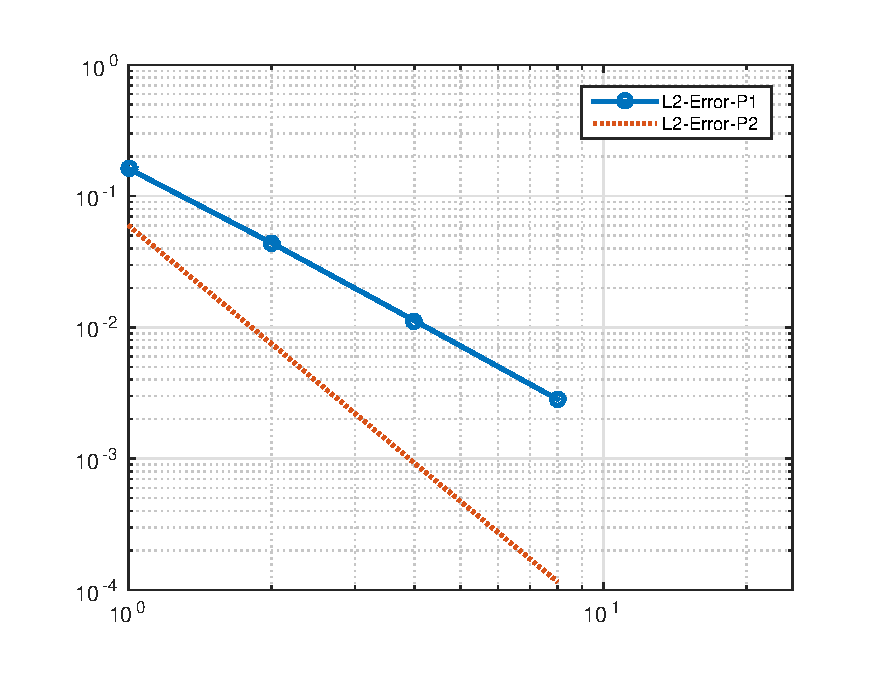
\includegraphics[width=.45\textwidth ]{pictures/convL2}
            }
    \caption{$H^1$ norm (left) and $L^2$ norm (right) vs mesh size for $ r =1,\, 2$.}
    \label{fig:normHL}
\end{figure}



% Stokes problem : stationary lid-driven cavity

\section{The Stokes Problem}
\label{sec:stokesproblem}
%
%
% SUMMARY:
% USAGE:
%
% AUTHOR:       Gilles Fourestey
% ORG:          EPFL
% E-MAIL:       foureste@iacspc.epfl.ch
%
% ORIG-DATE: 24-Nov-08 at 14:03:21
% LAST-MOD: 16-Aug-12 at 17:00:00 by Hélène Ruffieux
%
% DESCRIPTION:
% DESCRIP-END.


Let us consider flow of a viscous and incompressible fluid described by its velocity $u$
and pressure $p$. Its flow can be described, at low Reynolds number, by the Oseen Problem 

\begin{equation} \label{eqn-oseen}
\left\{
\begin{array}{lcl}
\displaystyle \alpha\, \bm{u} + \bm{\beta} \cdot \nabla \bm{u} - \nu \Delta \bm{u} +
\nabla p & = \bm{f}& \mbox{in}\; \Omega \\
\displaystyle \nabla \cdot \bm{u} & = 0& \mbox{in}\; \Omega  \\
\end{array}
\right.
\end{equation}

\noindent completed with suitable boundary conditions. Here $\Omega\subset \R^d$ ($d=1, 2, 3$) is the domain occupied by the fluid and $\nu$ is the kinematic viscosity of the fluid. If we set the convective
acceleration $\bm{\beta}$ and $\alpha$ to zero, we get the Stokes equations

\begin{equation} \label{eqn-stokes}
\left\{
\begin{array}{lcl}
- \nu \Delta \bm{u}+
\nabla p & = \bm{f}& \mbox{in}\; \Omega \\
\displaystyle \nabla \cdot \bm{u} & = 0 & \mbox{in}\; \Omega\,. \\
\end{array}
\right.
\end{equation}

We want to solve the following Stokes problem

\begin{equation} \label{eqn-stokes}
\left\{
\begin{array}{llll}
\displaystyle - \nu \Delta \bm{u}+
\nabla p & =& \bm{f} & \mbox{in } \Omega \\
\displaystyle \nabla \cdot \bm{u} & =& 0  & \mbox{in } \Omega \\
\bm{u} & =& (1, 0, 0) & \mbox{on } \partial \Omega_0 \\
\bm{u} & =& (0, 0, 0) & \mbox{on } \partial \Omega_1  \\
\bm{u} \cdot \bm{n} & =& 0 & \mbox {on } \partial \Omega_2\\
\end{array}
\right.
\end{equation}

\noindent where $\bm{n}$ is the normal unit vector to the domain boundary. The considered 3D domain $\Omega$ is represented by 

\vspace{0.5cm}
\begin{center}
\input cavityFigure.pdf_t
\end{center}
\vspace{0.5cm}

Writing $\Gamma_D = \partial \Omega_0 \cup \partial\Omega_1$ and $H^1_{\Gamma_D}(\Omega) = \{\bm{v}\in H^1(\Omega) : \bm{v}=\bm{0} \mbox{ on }\Gamma_D\}$, 
we can introduce the bilinear forms 
\begin{eqnarray*}
\displaystyle \forall\, \bm{u},\bm{v} \in \left(H^1(\Omega)\right)^3 & : &
a(\bm{u},\bm{v}) = \nu \int_{\Omega}\nabla \bm{u} \cdot \nabla \bm{v} dx\\
\displaystyle \forall\, \bm{v} \in \left(H^1(\Omega)\right)^3,\mbox{ } q \in L^2(\Omega) & : &
b(\bm{v},q) = \int_{\Omega} q\nabla \cdot \bm{v} dx \,.\\
\end{eqnarray*}
In variational form, the system (\ref{eqn-stokes}) thus reads: find $\bm{u}_0 \in \left(H^1_{\Gamma_D}(\Omega)\right)^3$ et $p \in
L^2(\Omega)$ such that
\begin{equation} \label{eqn-varia}
\left\{
\begin{array}{rlr}
\displaystyle a(\bm{u}_0,\bm{v}) + b(\bm{v},p) & =  \int_\Omega \bm{f}\cdot\bm{v}dx \,+\, \langle F^0, \bm{v} \rangle
& \hspace{1cm} \forall\, \bm{v} \in \left(H^1_{\Gamma_D}(\Omega)\right)^3 \\
b(\bm{u},q) & = \langle G^0, q \rangle & \hspace{1cm} \forall\, q \in L^2(\Omega)
\end{array}
\right.
\end{equation}
%find $u_h \in X_h$ and $p_h \in M_h$ so that,
where $F^0$ et $G^0$ are terms due to non-homogeneous Dirichlet boundary conditions on $\partial \Omega_0$. \\

In order to solve (\ref{eqn-varia}) using \lifev, let us create a working directory \verb+cavity_stokes+ in the directory \verb+ <lifev directory>/lifev/navier_stokes/examples/+ and get the following files:
 
\begin{itemize}
\item CMakeLists.txt
\item cavity\_stokes.cpp
\item data\_stokes
\end{itemize}

%The library has evolved much during the last years and you will find a few differences between the 
%instructions explained here and the \verb!cavity.cpp! code updated by 
%Gwenol Grandperrin in October of 2010. 
%
%
%Let's have a look a the makefile \ixns{Makefile}{GNU Makefile}.
%
%\begin{verbatim}
%# path to the compiler
%CC               = /usr/bin/g++
%
%SOURCES          = cavity.cpp
%OBJECTS          = $(SOURCES:.cpp=.o)
%EXECUTABLE       = cavity
%
%LIFELIBPATH      = -L<lifev lib directory path>
%LIFELIBS         = -llifefilters -llifesolver -llifefem \
%                   -llifealg -llifearray -llifecore -llifemesh
%LIFEINCLUDEPATH  = -I<lifev include directory path>
%
%TRILLIBPATH      = -L<trilinos lib directory path>
%TRILLIBS         = -laztecoo -laztecoo -ltriutils -lml \
%                   -lifpack -lamesos -lepetraext -lepetra \
%                   -lteuchos  -llapack -lblas
%TRILINCLUDEPATH  = -I<trilinos include directory path>
%
%# type "mpicxx -show" to get an hint of the contents of
%# the following variables
%MPILIBPATH       = -L<mpi lib directory path>
%MPILIBS          = -lmpi_cxx -lmpi -lopen-rte
%MPIINCLUDEPATH   = -I<mpi include directory path>
%
%METISLIBPATH	 = -L<parmetis lib directory path>
%METISLIBS        = -lparmetis -lmetis
%METISINCLUDEPATH = -I<parmetis include directory path>
%
%# uncomment this part for optimized compilation
%LDFLAGS         = -g0 -O2 -DTHREEDIM -lm
%# uncomment this part for debugging
%#LDFLAGS         = -g2 -O0 -DTHREEDIM -lm
%
%
%all: $(OBJECTS) $(EXECUTABLE)
%
%$(OBJECTS): $(SOURCES)
%	$(CC) $(LDFLAGS) \
%	$(MPIINCLUDEPATH) $(TRILINCLUDEPATH) $(LIFEINCLUDEPATH) \
%	$(SOURCES) -o $@
%
%$(EXECUTABLE): $(OBJECT)
%	echo "compiling the executable ... "
%	$(CC) $(CFLAGS) \
%	$(OBJECTS) $< -o $@ \
%	$(LIFELIBPATH) $(LIFELIBS) $(LIFEINCLUDEPATH) \
%	$(TRILLIBPATH) $(TRILLIBS) $(TRILINCLUDEPATH) \
%	$(METISPATH) $(METISLIBS) $(METISINCLUDE) \
%	$(MPILIBPATH) $(MPILIBS) $(MPIINCLUDEPATH) \
%
%
%clean:
%	rm -rf *o cavity
%
%\end{verbatim}
%

%You will need to fill the \verb|<...>| with your local
%configuration paths. You can also change the \verb|LDFLAGS| options in order to
%compile using the debug or the optimized mode in the g++ compiler. More information
%about using makefiles is available at \url{http://www.gnu.org/software/make/manual/make.html}.


We first draw attention to the fact that the top-level directory \verb+examples+ contains also a CMakeLists.txt file:
\begin{verbatim}
INCLUDE(TribitsAddExecutableAndTest)
INCLUDE(AddSubdirectories)

ADD_SUBDIRECTORIES(
  cavity_ns
  cavity_stokes
  cylinder
  oseen_assembler
)
\end{verbatim}

\noindent The last instructions recurse into the subdirectories. This does not actually cause another cmake executable to run.\\
\indent Let's then have a look at the CMakeLists.txt file created in our working subdirectory \verb!cavity_stokes!:

\begin{verbatim}
INCLUDE(TribitsAddExecutable)

# Add executable called "cavity_stokes_test" that is built from the source files
# "cavity_stokes.cpp". (Note that the name of the executable has to be uniquely chosen.) 
TRIBITS_ADD_EXECUTABLE(
  cavity_stokes_test
  SOURCES cavity_stokes.cpp
  COMM serial mpi
  )

# Access the data
TRIBITS_COPY_FILES_TO_BINARY_DIR(
  data_cavity_stokes_test
  SOURCE_FILES data
  SOURCE_DIR ${CMAKE_CURRENT_SOURCE_DIR}
)

# Access the mesh
TRIBITS_COPY_FILES_TO_BINARY_DIR(
  meshes_cavity_stokes_test
  SOURCE_FILES cube4x4.mesh
  SOURCE_DIR ${CMAKE_SOURCE_DIR}/lifev/core/data/mesh/freefem/
)
\end{verbatim}

\noindent More information about using cmake is available at \url{http://www.cmake.org/cmake/help/help.html}.\\  \indent We can now look at the sources contained in the file cavity\_stokes.cpp. We first include all the useful header files:

\begin{verbatim}
#include <lifev/core/LifeV.hpp>
#include <lifev/core/util/LifeChrono.hpp>
#include <lifev/core/array/MapEpetra.hpp>
#include <lifev/core/mesh/MeshData.hpp>
#include <lifev/core/mesh/MeshPartitioner.hpp>
#include <lifev/core/fem/FESpace.hpp>
#include <lifev/navier_stokes/solver/OseenData.hpp>
#include <lifev/navier_stokes/solver/OseenSolver.hpp>
#include <lifev/core/filter/ExporterEnsight.hpp>
#include <lifev/core/filter/ExporterHDF5.hpp>
#include <lifev/core/filter/ExporterEmpty.hpp>

// Trilinos-MPI communication definitions
#include <Epetra_ConfigDefs.h>
#ifdef HAVE_MPI
#include "Epetra_MpiComm.h"
#else
#include "Epetra_SerialComm.h"
#endif
\end{verbatim}

\noindent The last part is mandatory in order to define the Epetra Communicators (that contain the MPI calls) and should be at the begining of each program.\\
\indent The following instruction allows to use LifeV objects without refering to LifeV:: everytime.
Without it, we have to write LifeV::RefFE instead of just RefFE for instance.

\begin{verbatim}
using namespace LifeV;
\end{verbatim}

We introduce some typedef declarations to assign more pratical denominations to existing types and we label the different parts of our domain $\Omega$ to be able to apply later the boundary conditions.

\begin{verbatim}
typedef RegionMesh<LinearTetra>                 mesh_Type;
typedef OseenSolver< mesh_Type >                fluid_Type;
typedef fluid_Type::vector_Type                 vector_Type;
typedef std::shared_ptr<vector_Type>          vectorPtr_Type;    // Pointer
typedef FESpace< mesh_Type, MapEpetra >         feSpace_Type;
typedef std::shared_ptr<feSpace_Type>         feSpacePtr_Type;   // Pointer

const int BACK   = 1;
const int FRONT  = 2;
const int LEFT   = 3;
const int RIGHT  = 4;
const int BOTTOM = 5;
const int TOP    = 6;
\end{verbatim}



We next define real functions that will be used in the boundary condition
object.


\begin{verbatim}
Real lidBC(const Real& /*t*/,
           const Real& /*x*/, const Real& /*y*/, const Real& /*z*/,
           const ID& i)
{
    switch (i)
    {
    case 1:
        return 1.0;
    default:
        return 0.0;
    }
}

Real fZero( const Real& /* t */,
            const Real& /* x */, const Real& /* y */, const Real& /* z */,
            const ID& /* i */ )
{
    return 0.0;
}
\end{verbatim}

More generally speaking, boundary conditions functions must be defined using the following scheme:

\begin{verbatim}
Real function_name ( const Real& time,
                     const Real& x, const Real& y, const Real& z,
                     const ID&   id )
\end{verbatim}
\noindent where
\verb|time|
is the simulation time,
\verb|x, y, z|
are the space coordinates, and
\verb|ID|
is the component of the variable we want to set.
In our example, we want to set $(u_x, u_y, u_z) = (1, 0, 0)$ when we are in ${\partial \Omega}_0$
Therefore, when the ID is 1, i.e $x$, we return 1. For every other cases, i.e $y$ and $z$,
we return 0.\\

We can now proceed to the main block of the code.

\begin{verbatim}
int main(int argc, char** argv)
{
#ifdef HAVE_MPI
    MPI_Init(&argc, &argv);
#endif

    std::shared_ptr<Epetra_Comm>   comm;
#ifdef EPETRA_MPI
    comm.reset( new Epetra_MpiComm( MPI_COMM_WORLD ) );
    int nproc;
    MPI_Comm_size(MPI_COMM_WORLD, &nproc);
#else
    comm.reset( new Epetra_SerialComm() );
#endif
\end{verbatim}

\noindent These part will initialize the MPI process and create an Epetra communicator
that will be used throughout the code for message passing. See
%\begin{itemize}
%\item 
\url{http://www-unix.mcs.anl.gov/mpi/www/www3/MPI\_Init.html}
%\item \url{http://trilinos.sandia.gov/packages/docs/r6.0/packages/epetra/doc/html/classEpetra\_MpiComm.html}
%\end{itemize}
for more explanations.\\

The next block, although not necessarily in the comprehension of the FE resolution code, explains
how to manage output from a parallel code. As we do not want every processor to output
every piece of information, we set a master processor that will display relevant
pieces of information on the console ($0$ in our case).

\begin{verbatim}

    bool verbose(false);
    if (comm->MyPID() == 0)
    {
        verbose = true;
        std::cout << "[Initilization of MPI]" << std::endl;
#ifdef HAVE_MPI
        std::cout << "Using MPI (" << nproc << " proc.)" << std::endl;
#else
        std::cout << "Using serial version" << std::endl;
#endif
    }
\end{verbatim}

\noindent Then, a GetPot object (\url{http://getpot.sourceforge.net/}) is created
and is linked to a data description file using  the ``-f'' or ``--file'' parameters after
the main program name. By default (i.e. if no name is given) ``data'' is selected.

\begin{verbatim}
    if (verbose) std::cout << std::endl << "[Loading the data]" << std::endl;
    GetPot command_line(argc,argv);
    const std::string dataFileName = command_line.follow("data", 2, "-f","--file");
    GetPot dataFile(dataFileName);
\end{verbatim}

\noindent This GetPot object is used to store values like:
\begin{itemize}
\item the mesh name,
\item the time step (if any),
\item the discretization order,
\item the physics of the model,
\item the solver information,
\item ...
\end{itemize}

\begin{table}
\begin{center}
\begin{tabular}{|l|l|l|}
\hline
Name & Options & Description \\
\hline \hline
mesh\_dir & & mesh directory path \\ \hline
mesh\_file & & mesh file name \\ \hline
timestep & & problem time step \\ \hline
vel\_order & P1 & velocity discretization order \\ \
& P1Bubble & \\
& P2 & \\ \hline
press\_order & P1 & pressure discretization order \\
& P2 & \\ \hline
BDF\_order & 1 & time discretization order \\
& 2 & \\ \hline
\end{tabular}
\end{center}
\caption{Description of the discretization parameters
%\ixt{Fluid discretization parameters}{Fluid discretization}
}
\label{table-bcparams}
\end{table}

You can browse the default data file in every testsuite directory to see examples.
In general the entries
are filled with a default value if not specified,
but some entries are obligatory (like the mesh name for instance). \\
 We then create the mesh object and split it between processors

\begin{verbatim}
    if (verbose) std::cout << std::endl << "[Loading the mesh]" << std::endl;
    MeshData meshData;
    meshData.setup(dataFile, "fluid/space_discretization");
    if (verbose) std::cout << "Mesh file: " << meshData.meshDir() 
    					                             << meshData.meshFile() << std::endl;
    std::shared_ptr< mesh_Type > fullMeshPtr(new mesh_Type);
    readMesh(*fullMeshPtr, meshData);
    MeshPartitioner< mesh_Type >   meshPart(fullMeshPtr, comm);
\end{verbatim}


\noindent \lifev partitions meshes on the fly
using the parMetis library, that means that you do not have to provide the partitioned mesh in
order to have the simulation running.
\noindent In our case, after the call to the \verb!MeshPartitioner!  constructor, \verb!meshPart! will store
the local part of the mesh. Using this local mesh, 
we can create our Finite Element spaces:

\begin{verbatim}
    if (verbose) std::cout << std::endl << "[Creating the FE spaces]" << std::endl;
    std::string uOrder =  dataFile( "fluid/space_discretization/vel_order",   "P2");
    std::string pOrder =  dataFile( "fluid/space_discretization/press_order", "P1");
    
    if (verbose) std::cout << "FE for the velocity: " << uOrder << std::endl
                               << "FE for the pressure: " << pOrder << std::endl;
    if (verbose) std::cout << "Building the velocity FE space... " << std::flush;
    feSpacePtr_Type uFESpacePtr( new feSpace_Type(meshPart, uOrder, 3, comm) );
    if (verbose) std::cout << "ok." << std::endl;

    if (verbose) std::cout << "Building the pressure FE space... " << std::flush;
    feSpacePtr_Type pFESpacePtr( new feSpace_Type(meshPart,pOrder,1,comm) );
    if (verbose) std::cout << "ok." << std::endl;

    // Total degrees of freedom (elements of matrix)
    UInt totalVelDof   = uFESpacePtr->map().map(Unique)->NumGlobalElements();
    UInt totalPressDof = pFESpacePtr->map().map(Unique)->NumGlobalElements();
\end{verbatim}

\noindent The constructor called for the instances of the FESpace class takes as arguments

\begin{itemize}
\item the mesh,
\item the chosen elements type (here we decided to use P2/P1 elements),
\item the fields dimension,
\item the MPI communicator.
\end{itemize}

Let's continue with the specification of the boundary conditions on all our boundary faces. BCHandler is the class that stores the boundary conditions. Here is the prototype of the \verb!addBC! function that we use for the assignment.
\small
\begin{verbatim}
//! add new BC to the list (user defined function)
/*!
\param name the name of the boundary condition
\param flag the mesh flag identifying the part of the mesh where the boundary condition applies
\param type the boundary condition type: Natural, Essential, Robin
\param mode the boundary condition mode: Scalar, Full, Component, Normal, Tangential
\param bcf the function holding the user defined function involved in this boundary condition
\param std::vector<ID> storing the list of components involved in this boundary condition
*/
void addBC( const std::string&     name,
            const EntityFlag&      flag,
            const bcType_Type&     type,
            const bcMode_Type&     mode,
            BCFunctionBase&        bcf,
            const std::vector<ID>& comp );
\end{verbatim}
\normalsize
\verb!name! is a boundary condition description string,
\verb!flag! is the boundary condition number as defined in the mesh,
\verb!mode! is the mode, \verb!bcf! is the function holding the user-defined function involved
in the boundary condition. Moreover, \verb!type! and \verb!mode! are respectively the boundary condition type
and mode. Please refer to the table (\ref{table-bcparams}) for a description of their values.
Finally, \verb!comp! is a vector storing the components in the boundary condition.\\

\begin{table}
\begin{center}
\begin{tabular}{|l|l|l|}
\hline
Name & Options & Description \\
\hline \hline
type &  Natural & Neumann\\
& Essential & Dirichlet \\
& Robin&\\

\hline
mode & Scalar & 1 dimension BC \\
& Full & 3 component BC \\
& Component  & Separate component BC \\
& Normal & Normal BC \\
& Tangential & Tangential BC \\
\hline

\end{tabular}
\end{center}
\caption{ Boundary Condition parameters description
%\ixt{Boundary Conditions parameters}{Boundary Conditions}
}
\label{table-bcparams}
\end{table}



In our example, we recall that we have to set essential boundary conditions on the top face, $\bm{u}=(1,0,0)$, and on the left, right and bottom faces, $\bm{u}=(0,0,0)$. We have:
\begin{verbatim}
    if (verbose) std::cout<< std::endl << "[Boundary conditions]" << std::endl;

    BCFunctionBase uZero(fZero);
    BCFunctionBase uLid(lidBC);

    BCHandler bcH;
    bcH.addBC( "Top"   , TOP   , Essential, Full, uLid , 3 );
    bcH.addBC( "Left"  , LEFT  , Essential, Full, uZero, 3 );
    bcH.addBC( "Right" , RIGHT , Essential, Full, uZero, 3 );
    bcH.addBC( "Bottom", BOTTOM, Essential, Full, uZero, 3 );
\end{verbatim}

For the front and back faces, we have natural boundary conditions, $\bm{u}\cdot \bm{n}=0$. Note however that this means
\begin{equation*}
u_x = 0 \mbox{ for } x=1, L
\end{equation*}
(since the two concerned planes are defined by $x = 0$ and $x = L$).
So in order to set our first component, \verb!x!, we define the vector

\begin{verbatim}
    std::vector<ID> xComp(1);
    xComp[0] = 1;
\end{verbatim} 



\noindent Then, we add an essential boundary condition on the x-component by calling
\begin{verbatim}
    bcH.addBC( "Back"  , BACK  , Essential, Component, uZero, xComp );
    bcH.addBC( "Front" , FRONT , Essential, Component, uZero, xComp );
\end{verbatim}

\noindent This will set a null function to the first component on the front and back faces. We could have just easily defined
another function for the others components using the same procedure.

We also mention that we have also the possibility to apply Flux boundary conditions. Here is the procedure that we can use:

\begin{verbatim}

    // Get the number of Lagrange Multiplyers (LM) and set the offsets
    std::vector<bcName_Type> fluxVector = bcH.findAllBCWithType( Flux );
    UInt numLM = static_cast<UInt>( fluxVector.size() );

    UInt offset = uFESpacePtr->map().map(Unique)->NumGlobalElements()
                         + pFESpacePtr->map().map(Unique)->NumGlobalElements();

    for ( UInt i = 0; i < numLM; ++i )
        bcH.setOffset( fluxVector[i], offset + i );
\end{verbatim}

\noindent In our case, we simply note that \verb|numLM = 0| and so the loop is not entered.\\

Now we build the solver. In \lifev,
a solver has the following properties:
\begin{itemize}
\item it builds and stores the linear FE matrices,
\item it builds the preconditioners,
\item it builds the linear solvers.
\end{itemize}
As our problem can be view as a special case of an Oseen system, we will first create and setup an object from a class, the \verb+OseenData+ class, designed to store and manage the related informations.

\begin{verbatim}
 if (verbose) std::cout<< std::endl << "[Creating the problem]" << std::endl;
    std::shared_ptr< OseenData > oseenData(new OseenData);
    oseenData->setup( dataFile );
\end{verbatim}    


Calling now the constructor of our solver will initialize the matrices, preconditioner and the linear solver
but neither will be fully constructed. Instead, the matrices will be initialized using the
velocity and pressure FE spaces


\begin{verbatim}
    // The problem (matrix and rhs) is packed in an object called fluid
    OseenSolver< mesh_Type > fluid (oseenData, *uFESpacePtr, *pFESpacePtr,
                                     comm, numLM);                       
\end{verbatim}

Now that the class has been instantiated, we need to set it up with the data file parameters

\begin{verbatim}
    // Gets inputs from the data file
    fluid.setUp(dataFile);
\end{verbatim}
    
\noindent Calling \verb|setUp|
will basically build the preconditioner and the linear solver using the AztecOO 
options\footnote{see \url{http://trilinos.sandia.gov/packages/docs/r9.0/packages/aztecoo/doc/html/classAztecOO.html} for more information.}
contained in the data file.   


\begin{table}
\begin{center}
\begin{tabular}{|l|l|}
\hline
name & options\\
\hline \hline
solver & cg \\
& cg\_condnum\\
& gmres (default)\\
& gmres\_condnum\\
& cgs\\
& tfqmr\\
& bicgstab\\
\hline
conv & r0\\
& rhs (default) \\
& Anorm  \\
& noscaled  \\
& sol \\
\hline

precond & none (default) \\
& none \\
&Jacobi \\
&Neumann \\
&ls \\
&sym\_GS \\
&dom\_decomp \\
\hline

scaling & none (default) \\
&    Jacobi \\
&    BJacobi \\
&    row\_sum \\
&    sym\_diag \\
&    sym\_row\_sum \\
&    equil \\
&    sym\_BJacobi \\

\hline

tol   & default : 1e-6  \\

\hline

kspace & default : 30  \\

\hline

max\_iter & default : 500  \\

\hline

drop\_tol & default : 0. \\

\hline

\end{tabular}
\end{center}
\caption{Main parameters for the Trilinos solver}
\label{table-solveroptions}
\end{table}

Then we can build the linear system (assemble the matrices):
\begin{verbatim}
    fluid.buildSystem();
\end{verbatim}

\noindent It will create the full finite element linear matrix. Note that, despite the fact
that we passed both the velocity and the pressure FE spaces, the solver will consider
only one finite element constructed by performing a direct sum of the two FE spaces.
The associated ``full'' map can be retrieved using the \verb|getMap| method. 

\begin{verbatim}
     // Communication map: 
    MapEpetra fullMap(fluid.getMap());
\end{verbatim}
\noindent It is useful to create vectors to store the solutions vector after the linear system is solved and before, to setup attributes of the \verb!fluid! object:  we set the right handside (\verb!rhs!) to zero. As we deal with a Stokes problem, there is also no mass matrix (\verb!alpha!) and no advection term (\verb!beta!). These are the three arguments needed to update the system in the Oseen class:\\

\begin{verbatim}
    vector_Type beta( fullMap );
    vector_Type rhs ( fullMap );
    double alpha=0.; // Stokes problem
    beta *= 0.;  // Stokes problem
    rhs  *= 0.;
    fluid.updateSystem(alpha,beta,rhs);
    fluid.iterate(bcH);
\end{verbatim}

 The last line will result in solving the system (\ref{eqn-stokes}) and we note that the member \verb!iterate! requires the boundary conditions
as parameters. More precisely, it will:
\begin{itemize}
\item build the full matrix,
\item apply the boundary conditions,
\item solve the system.
\end{itemize}

In \lifev, we mainly use Paraview in order to postprocess our problem solutions.
Writing a Paraview solution is quite straightforward using the ExporterHDF5 class.
%We call its constructor where we give the data file, the mesh and the filename of the solution file with references to the solution vector.

\begin{verbatim}
    std::shared_ptr< ExporterHDF5<mesh_Type> > exporter;
    std::string const exporterType =  dataFile( "exporter/type", "ensight");
    exporter.reset( new ExporterHDF5<mesh_Type> ( dataFile, "cavity_stokes_example" ) );
    exporter->setPostDir( "./" );  // This is a test to see if M_post_dir is working
    exporter->setMeshProcId( meshPart.meshPartition(), comm->MyPID() );
\end{verbatim}

We have to define a variable that will store the solution:
\begin{verbatim}
    vectorPtr_Type velAndPressure;
    velAndPressure.reset( new vector_Type(*fluid.solution(), exporter->mapType() ) );
\end{verbatim}

Finally, we add the variables to be saved:
\begin{verbatim}
    exporter->addVariable( ExporterData<mesh_Type>::VectorField, "velocity", 
                           uFESpacePtr, velAndPressure, UInt(0) );
    exporter->addVariable( ExporterData<mesh_Type>::ScalarField, "pressure", 
                           pFESpacePtr, velAndPressure, 
                           UInt(3*uFESpacePtr->dof().numTotalDof()) );
    exporter->postProcess( 0 );
    exporter->closeFile();
\end{verbatim}

The final statements stops the parallel part of the code and ends the main:
\begin{verbatim}
#ifdef HAVE_MPI
    MPI_Finalize();
#endif

    return 0;
}
\end{verbatim}

You must run the cavity\_stokes executable named \verb!cavity_stokes_example! using the command
\verb!mpirun -np procs cavity_stokes_example! where \verb!procs! is the number 
of processors you want to use for your computation.

You may now visualize the result using Paraview.


%\begin{verbatim}
%
%#include "Epetra_config.h"
%#include "Epetra_MpiComm.h"
%
%\end{verbatim}
%
%This part is mandatory in order to define the Epetra Communicators (that contain the MPI calls) 
% and should be
%at the begining of each program.
%
%
%\begin{verbatim}
%#include <boost/program_options.hpp>
%#include <life/lifecore/life.hpp>
%#include <life/lifecore/application.hpp>
%#include <life/lifearray/EpetraMatrix.hpp>
%#include <life/lifealg/EpetraMap.hpp>
%#include <life/lifemesh/partitionMesh.hpp>
%#include <life/lifesolver/OseenData.hpp>
%#include <life/lifefem/FESpace.hpp>
%#include <life/lifefem/bdfNS_template.hpp>
%#include <life/lifefilters/ensight.hpp>
%#include <life/lifesolver/OseenSolver.hpp>
%#include <iostream>
%\end{verbatim}


%
%\begin{verbatim}
%using namespace LifeV;
%\end{verbatim}
%
%Use this to use LifeV objects  without refering to LifeV:: everytime.
%Without it, we have to use LifeV::RefFE instead of just RefFE for instance.
%
%
%\begin{verbatim}
%typedef std::function<Real ( Real const&,
%                               Real const&,
%                               Real const&,
%                               Real const&,
%                               ID const& )> fct_type;
%
%typedef OseenSolver< RegionMesh<LinearTetra> >::vector_type  vector_type;
%typedef std::shared_ptr<vector_type>                   vector_ptrtype;
%
%Real zero_scalar( const Real& /* t */,
%                  const Real& /* x */,
%                  const Real& /* y */,
%                  const Real& /* z */,
%                  const ID& /* i */ )
%{
%    return 0.;
%}
%
%Real uLid(const Real& t, const Real& /*x*/, const Real& /*y*/, const Real& /*z*/, const ID& i)
%{
%  switch(i) {
%  case 1:
%    return 1.0;
%    break;
%  case 3:
%      return 0.0;
%      break;
%  case 2:
%      return 0.0;
%    break;
%  }
%  return 0;
%}
%
%\end{verbatim}
%
%In this section, we have defined real functions that will be used in the boundary condition
%object. Boundary conditions functions must be defined using the following scheme
%
%\begin{verbatim}
%
%Real function_name ( const Real& time,
%                     const Real& x, const Real& y, const Real& z,
%                     const ID&   id )
%
%\end{verbatim}
%
%where
%\verb|time|
%is the simulation time,
%\verb|x, y, z|
%are the space coodinates, and
%\verb|ID|
%is the component of the variable we want to set.
%In our example, we want to set $(u_x, u_y, u_z) = (1, 0, 0)$ when we are in ${\partial \Omega}_1$
%Therefore, when the ID is 1, i.e $x$, we return 1. For every other cases, i.e $y$ and $z$,
%we return 0. 
%
%We could have used another boundary condition, for instance 
%
%\begin{verbatim}\end{verbatim}
%\begin{verbatim}
%Real uLid(const Real& t, const Real& /*x*/, const Real& /*y*/, const Real& /*z*/, const ID& i)
%{
%  switch(i) {
%  case 1:
%      return x*(1 - x);
%      break;
%  case 3:
%      return 0.0;
%      break;
%  case 2:
%      return 0.0;
%      break;
%  }
%  return 0;
%}
%\end{verbatim}
%
%
%The main difference is that, using this functions, the boundary condition on ${\partial \Omega}_1$
%now becomes
%\begin{equation*}
%  u = (x(1 - x), 0, 0) \mbox{ on } {\partial \Omega}_0 \\
%\end{equation*}

%We can now proceed to the main block of the code.
%
%\begin{verbatim}
%int main( int argc, char** argv )
%{
%    MPI_Init(&argc, &argv);
%    Epetra_MpiComm comm(MPI_COMM_WORLD);
%
%\end{verbatim}
%
%These two lines will initialize the MPI process and create an Epetra communicator
%that will be used throughout the code for message passing. See
%\begin{itemize}
%\item \url{http://www-unix.mcs.anl.gov/mpi/www/www3/MPI\_Init.html}
%\item \url{http://trilinos.sandia.gov/packages/docs/r6.0/packages/epetra/doc/html/classEpetra\_MpiComm.html}
%\end{itemize}
%for more explanations.
%
%\begin{verbatim}
%    // a flag to see who's the master for output purposes
%    bool verbose = comm.MyPID() == 0;
%
%    if ( comm.MyPID() == 0 )
%        {
%            cout << "% using MPI" << endl;
%            int ntasks;
%            int err = MPI_Comm_size(MPI_COMM_WORLD, &ntasks);
%            std::cout << "My PID = " << comm.MyPID() << " out of "
%                      << ntasks << " running." << std::endl;
%        }
%\end{verbatim}
%This block, although not necessarily in the comprehension of the FE resolution code, explains
%how to manage output from a parallel code. As we do not want every processor to output
%every piece of information, we set a master processor that will display relevant
%pieces of information on the console ($0$ in our case).
%\begin{verbatim}
%
%    // Read from the data file. Its name can be given using the
%    // -f or --file argument after the name of launch program.
%    // By default, it's data.
%
%    GetPot command_line(argc, argv);
%    const std::string data_file_name = command_line.follow("data", 2, "-f", "--file");
%    GetPot dataFile( data_file_name );
%
%\end{verbatim}
%
%\noindent In this part, a GetPot object (http://getpot.sourceforge.net/) is created
%and is linked to a data description file using  the ``-f'' or ``--file'' parameters after
%the main program name. This GetPot object is used to store values like:
%\begin{itemize}
%\item the mesh name,
%\item the time step,
%\item the discretization order,
%\item the physics of the model,
%\item the solver information,
%\item ...
%\end{itemize}
%You can browse the default data file in every testsuite directory to see examples.
%In general the entries
%are filled with a default value if not specified,
%but some entries are obligatory, like the mesh name for instance. 
%
%A data object will be used to store this information. In our case, since we want to
%solve a Navier-Stokes problem, we need to use the OseenData object.
%Given the GetPot object we have just defined, it will parse the specified data file
%to retreive all the information necessary to run the simulation.
%
%\begin{verbatim}
%
%    // everything ( mesh included ) will be stored in a class
%    std::shared_ptr< DataTime > dataTime( new DataTime( dataFile ) );
%    std::shared_ptr< MeshData< RegionMesh<LinearTetra> > > meshData( new MeshData< RegionMesh<LinearTetra> >( dataFile ) );
%
%    OseenData<RegionMesh<LinearTetra> > oseenData( dataFile, dataTime, meshData );
%
%\end{verbatim}
%
%\begin{table}
%\begin{center}
%\begin{tabular}{|l|l|l|}
%\hline
%Name & Options & Description \\
%\hline \hline
%mesh\_dir & & mesh directory path \\ \hline
%mesh\_name & & mesh file name \\ \hline
%timestep & & problem time step \\ \hline
%vel\_order & P1 & velocity discretization order \\ \
%& P1Bubble & \\
%& P2 & \\ \hline
%press\_order & P1 & pressure discretization order \\
%& P2 & \\ \hline
%order\_bdf & 1 & time discretization order \\
%& 2 & \\ \hline
%\end{tabular}
%\end{center}
%\caption{ Description of the discretization parameters.
%%\ixt{Fluid discretization parameters}{Fluid discretization}
%}
%\label{table-bcparams}
%\end{table}
%
%
%\noindent After this line, everything we need to know about our problem is stored
%in oseenData.
%
%To build a FE solver for our cavity problem we need:
%\begin{itemize}
%\item a finite element space,
%\item the boundary conditions,
%\item a solver that will build and solve the linear system derived from our weak formulation.
%\end{itemize}
%
%\begin{verbatim}
%    // BCHandler is the class that stores the boundary conditions. Here we will
%    // set 3 boundary conditions:
%    // top               : (ux, uy, uz) = (1., 0., 0.) essential BC
%    // left, right, down : (ux, uy, uz) = (0., 0., 0.) essential BC
%    // front and rear    : uz = 0 essential BC
%
%    BCHandler bcH(3);
%
%    std::vector<ID> zComp(1);
%    zComp[0] = 3;
%
%    BCFunctionBase uIn  ( boost::bind(&uLid, std::placeholders::_1, std::placeholders::_2, std::placeholders::_3, std::placeholders::_4, std::placeholders::_5) );
%    BCFunctionBase uZero( zero_scalar );
%
%    // boundary conditions definition.
%    // the first two are classical essential or dirichlet conditions
%    bcH.addBC( "Upwall",   UPWALL,   Essential, Full,      uIn,   3 );
%    bcH.addBC( "Wall",     WALL,     Essential, Full,      uZero, 3 );
%\end{verbatim}
%
%Bondary conditions \ixv{Boundary Conditions} part. Here is the prototype of the \verb!addBC! function 
%
%\begin{verbatim}
%    //! add new BC to the list (user defined function)
%    /*!
%      \param name the name of the boundary condition
%      \param flag the mesh flag identifying the part of the mesh where the boundary condtion applies
%      \param type the boundary condition type: Natural, Essential, Robin
%      \param mode the boundary condition mode: Scalar, Full, Component, Normal, Tangential
%      \param bcf the function holding the user defined function involved in this boundary condition
%      \param std::vector<ID> storing the list of components involved in this boundary condition
%    */
%    void addBC( const std::string&     name,
%                const EntityFlag&      flag,
%                const bcType_Type&          type,
%                const bcMode_Type&          mode,
%                BCFunctionBase&        bcf,
%                const std::vector<ID>& comp );
%\end{verbatim}
%\verb!name! is a boundary condition description string,
%\verb!flag! is the boundary condition number as defined in the mesh (in this example, the variables \verb+UPWALL+
%and \verb+WALL+ are defined at the beginning of the file),
%\verb!mode! is the mode, \verb!bcf! is the function holding the user-defined function involved
%in the boundary condition. \verb!type! and \verb!mode! are respectively the boundary condition type
%and mode. Please refer to the table (\ref{table-bcparam}) for a description of their values.
%
%\begin{table}
%\begin{center}
%\begin{tabular}{|l|l|l|}
%\hline
%Name & Options & Description \\
%\hline \hline
%type &  Natural & Neumann\\
%& Essential & dirichlet \\
%& Robin\\
%
%\hline
%mode & Scalar & 1 dimension BC \\
%& Full & 3 component BC \\
%& Component  & Sepate compenent BC \\
%& Normal & Normal BC \\
%& Tangential & Tangential BC \\
%\hline
%
%\end{tabular}
%\end{center}
%\caption{ Boundary Condition parameters description
%%\ixt{Boundary Conditions parameters}{Boundary Conditions}
%}
%\label{table-bcparams}
%\end{table}
%
%\verb!comp! is a vector storing the components in the boundary condition.
%The last boundary condition we want to impose is 
%\verb!SLIPWALL! 
%( i.e $20$ in the mesh file, or $\partial \Omega_2$ in (\ref{eqn-stokes}) ), will get 
%a slipwall boundary condition, i.e
%\begin{equation}\label{eqn-slipwallbc}
%u \cdot n = 0
%\end{equation}
%This means, since the two concerned planes are defined by $z = 0$ and $z = L$, that
%\begin{equation*}
%u_z = 0 \mbox{ for } z=1,L
%\end{equation*}
%In order to set our third component (\verb!z!), we define the vector
%\begin{verbatim}
%    std::vector<ID> zComp(1);
%    zComp[0] = 3;
%\end{verbatim}
%Then, we add an essential (Dirichlet) boundary condition on the z component by calling
%\begin{verbatim}
%    bcH.addBC( "Slipwall", SLIPWALL, Essential, Component, uZero, zComp );
%\end{verbatim}
%This will set a null function to the third component on the slipwall. We could have just easily defined
%another function for the others components using the same procedure.
%
%Now we get the mesh \ixv{Mesh}. LifeV partitions meshes \ixns{Paritioning}{Mesh} on the fly
%using the parMetis library, that means that you do not have to provide the partitioned mesh in
%order to have the simulation running.
%
%\begin{verbatim}
%    // partitioning the mesh
%    partitionMesh< RegionMesh<LinearTetra> >
%             meshPart(*oseenData.meshData()->mesh(), comm);
%\end{verbatim}
%
%In our case, after the call to the \verb!partitionMesh! constructor, \verb!meshPart! will store
%the local part of the mesh. Using this local mesh, 
%we can create our Finite Element \ixns{Finite Element Space}{Finite Element} spaces.
%In \lifev, a Finite Element Space is a class storing:
%\begin{description}
%\item a mesh,
%\item a reference Finite Element,
%\item quadrature rules to integrate reference functions on the mesh elements or the boundaries.
%\end{description}
%
%A reference Finite Element in \lifev is a class containing the geometrical definition
%of the mesh elements and the polynomial approximation order we want to use.
%
%\begin{verbatim}
%    // Now we proceed with the FESpace definition
%    // here we decided to use P2/P1 elements
%
%    const RefFE*    refFE_vel;
%    const QuadRule* qR_vel;
%    const QuadRule* bdQr_vel;
%
%    refFE_vel = &feTetraP2;
%    qR_vel    = &quadRuleTetra15pt; // DoE 5
%    bdQr_vel  = &quadRuleTria3pt;   // DoE 2
%
%\end{verbatim}
%
%After these lines, \verb!refFE_vel! contains the desired reference finite element  
%\ixns{Reference Finite Element}{Finite Element}. See table \ref{table-feapproxorder}
%for the descrition of available parameters.
%
%\begin{table}
%\begin{center}
%\begin{tabular}{|l|l|l|}
%\hline
%Name  & Description \\
%\hline \hline
%feTetraP1 & P1 finite element on Tetrahedron \\
%feTetraP1Bubble & P1-Bubble finite element on Tetrahedron \\
%feTetraP2 & P2 finite element on Tetrahedron \\
%\hline
%\end{tabular}
%\end{center}
%\caption{ Reference Finite Element parameters}
%\label{table-feapproxorder}
%\end{table}
%
%Quadrature rules \ixv{Quatrature Rules} are defined according the polynomial order we have defined.
%
%\begin{table}
%\begin{center}
%\begin{tabular}{|l|l|l|}
%\hline
%Name  & Description & exact p. order\\
%\hline \hline
%quadRuleTetra1pt   & 1 point & 1 \\
%quadRuleTetra3pt   & 3 point & 2 \\
%quadRuleTetra5pt   & 5 point &   \\
%quadRuleTetra15pt  & 15 point &  \\
%quadRuleTetra64pt  & 64 point &  \\
%\hline
%\end{tabular}
%\end{center}
%\caption{ Quadrature Rule description}
%\label{table-feapproxorder}
%\end{table}
%
%Everything is ready to create our Finite Element space
%
%\begin{verbatim}
%    // Everything is ready to build the FE space
%    // first the velocity FE space
%
%    if (verbose)
%        std::cout << "Building the velocity FE space ... " << std::flush;
%
%    FESpace< RegionMesh<LinearTetra>, EpetraMap > uFESpace(meshPart,
%                                                             *refFE_vel,
%                                                             *qR_vel,
%                                                             *bdQr_vel,
%                                                             3,
%                                                             comm);
%
%\end{verbatim}
%
%We define the reference finite element as P2 and two quadrature rules: one general and one
%for the boundary integration. Once these classes are defined, we call the FE space
%object constructor with the following input parameters:
%\begin{itemize}
%\item meshPart is the local partioned mesh,
%\item *refFE\_vel is the reference finite element,
%\item *qR\_vel and *bdQR\_vel are the quadrature rules,
%\item 3 is the field dimension,
%\item comm is the MPI communicator.
%\end{itemize}
%
%Of course, we do the same with the pressure. This time, we use a P1 discretization
%
%\begin{verbatim}
%
%    const RefFE*    refFE_press;
%    const QuadRule* qR_press;
%    const QuadRule* bdQr_press;
%
%    refFE_press = &feTetraP1;
%    qR_press    = &quadRuleTetra4pt;  // DoE 2
%    bdQr_press  = &quadRuleTria3pt;   // DoE 2
%
%    if (verbose)
%        std::cout << "Building the pressure FE space ... " << std::flush;
%
%    FESpace< RegionMesh<LinearTetra>, EpetraMap > pFESpace(meshPart,
%                                                             *refFE_press,
%                                                             *qR_press,
%                                                             *bdQr_press,
%                                                             1,
%                                                             comm);
%
%\end{verbatim}
%
%Now we build the solver. In \lifev,
%a solver has the following properties:
%\begin{itemize}
%\item it builds and stores the linear FE matrices,
%\item it builds the preconditioners,
%\item it builds the linear solvers.
%\end{itemize}
%
%Calling the constructor will initialize the matrices, preconditioner and the linear solver
%but neither will be fully constructed. Instead, the matrices will be initialized using the
%velocity and pressure FE spaces
%
%\begin{verbatim}
%
%    // now that the FE spaces are built, we proceed to the NS solver constrution
%    // we use the oseen class
%
%    if (verbose) std::cout << "Calling the fluid constructor ... ";
%
%    OseenSolver< RegionMesh<LinearTetra> > fluid (oseenData,
%                                              uFESpace,
%                                              pFESpace,
%                                              comm);
%
%
%\end{verbatim}
%
%Now that the class has been instantiated, we need to set it up with the data file parameters
%
%\begin{verbatim}
%    // Now, the fluid solver is set up using the data file
%    fluid.setUp(dataFile);
%\end{verbatim}
%
%Calling \verb|setUp|
%will basically build the preconditioner and the linear solver using the AztecOO 
%options \footnote{see \url{http://trilinos.sandia.gov/packages/docs/r9.0/packages/aztecoo/doc/html/classAztecOO.html} for more information}
%contained in the data file.
%
%\begin{table}
%\begin{center}
%\begin{tabular}{|l|l|}
%\hline
%name & options\\
%\hline \hline
%solver & cg \\
%& cg\_condnum\\
%& gmres (default)\\
%& gmres\_condnum\\
%& cgs\\
%& tfqmr\\
%& bicgstab\\
%\hline
%conv & r0\\
%& rhs (default) \\
%& Anorm  \\
%& noscaled  \\
%& sol \\
%\hline
%
%precond & none (default) \\
%& none \\
%&Jacobi \\
%&Neumann \\
%&ls \\
%&sym\_GS \\
%&dom\_decomp \\
%\hline
%
%scaling & none (default) \\
%&    Jacobi \\
%&    BJacobi \\
%&    row\_sum \\
%&    sym\_diag \\
%&    sym\_row\_sum \\
%&    equil \\
%&    sym\_BJacobi \\
%
%\hline
%
%tol   & default : 1e-6  \\
%
%\hline
%
%kspace & default : 30  \\
%
%\hline
%
%max\_iter & default : 500  \\
%
%\hline
%
%drop\_tol & default : 0. \\
%
%\hline
%
%\end{tabular}
%\end{center}
%\caption{Main parameters for the Trilinos solver}
%\label{table-solveroptions}
%\end{table}
%
%%See \url{
%%http://trilinos.sandia.gov/packages/aztecoo/AztecOOUserGuide.pdf} for more information).
%Then we can build the linear system
%\begin{verbatim}
%    // then we build the constant matrices
%    fluid.buildSystem();
%\end{verbatim}
%
%This will create the full finite element linear matrix. Note that, despite the fact
%that we passed both the velocity and the pressure FE spaces, the solver will consider
%only one finite element constructed by performing a direct sum of the two FE spaces.
%The associated ``full'' map can be retrieved using the \verb|getMap| method 
%
%\begin{verbatim}
%    // this is the total map ( velocity + pressure ). it will be used to create
%    // vectors to store the solutions
%
%    EpetraMap fullMap(fluid.getMap());
%
%    if (verbose) std::cout << "ok." << std::endl;
%\end{verbatim}
%
%Using this map is obligatory when we access the solution vector after the linear system is solved.\\
%
%In \lifev, we mainly use Paraview in order to postprocess our problem solutions.
%Writing a Paraview solution is quite straightforward using the Ensight class.
%We call the Ensight constructor where we give the data file, the mesh and the filename of the solution file
%with references to the solution vector.
%
%\begin{verbatim}
%
%    // finally, let's create an exporter in order to view the results
%    // here, we use the ensight exporter
%
%    Ensight<RegionMesh<LinearTetra> >
%           ensight( dataFile, meshPart.mesh(), "cavity", comm.MyPID());
%
%    // we have to define a variable that will store the solution
%    vector_ptrtype velAndPressure ( new vector_type(fluid.solution(),
%                                                    Repeated ) );
%
%    // and we add the variables to be saved
%    // the velocity
%    ensight.addVariable( ExporterData::Vector, "velocity", velAndPressure,
%                         UInt(0), uFESpace.dof().numTotalDof() );
%
%    // and the pressure
%    ensight.addVariable( ExporterData::Scalar, "pressure", velAndPressure,
%                         UInt(3*uFESpace.dof().numTotalDof()),
%                         UInt(3*uFESpace.dof().numTotalDof() +
%                                pFESpace.dof().numTotalDof()) );
%
%    // a little barrier to synchronize the processes
%    MPI_Barrier(MPI_COMM_WORLD);
%\end{verbatim}
%
%%Here is the occasion to introduce an important concept in \lifev/Trilinos (...).
%
%We are now set for the solution of the linear system.
%
%\begin{verbatim}
%
%    vector_type beta( fullMap );
%    vector_type rhs ( fullMap );
%
%    beta        *= 0.;
%    rhs         *= 0.;
%
%    double alpha = 0.;
%\end{verbatim}
%
%Using the full map defined above, we set the advection term and right handside to zero.
%
%\begin{verbatim}
%    // updating the system with no mass matrix, advection and rhs set to zero,
%    // that is the stokes problem
%    fluid.updateSystem(alpha, beta, rhs );
%\end{verbatim}
%
%In the Oseen class, \verb|updateSystem| has 3 arguments:
%\begin{itemize}
%\item \verb|alpha| is the coefficient in front of the mass term,
%\item \verb|beta| is the advection term,
%\item \verb|rhs| is the righthand side.
%\end{itemize}
%
%Setting these 3 terms to zero will result in solving the system (\ref{eqn-stokes}).
%The linear system is solved by calling \verb!iterate!, which requires the boundary conditions
%as parameters. The member \verb!iterate! will:
%\begin{itemize}
%\item build the full matrix,
%\item apply the boundary conditions,
%\item solve the system.
%\end{itemize}
%
%\begin{verbatim}
%    // iterating the solver in order to produce the solution
%    fluid.iterate( bcH );
%
%    // a little postprocessing to see if everything goes according to plan
%    *velAndPressure = fluid.solution();
%    ensight.postProcess( 0 );
%
%\end{verbatim}
%
%You must run the cavity executable named \verb!cavity_example! using 
%\verb!mpirun -np procs cavity_example! where \verb!procs! is the number 
%of processors you want to use for your computation. 
%
%
%
%You may now visualize the result using Paraview.
%
%%
%%%%%%%%%%%%%% Some Settings for emacs and auc-TeX
%% Local Variables:
%% TeX-master: t
%% TeX-command-default: "PDFLaTeX"
%% TeX-parse-self: t
%% TeX-auto-save: t
%% x-symbol-8bits: nil
%% TeX-auto-regexp-list: TeX-auto-full-regexp-list
%% eval: (ispell-change-dictionary "american")
%% End:
%%


% Navier Stokes problem

\section{The Navier-Stokes Problem}
\label{sec:navierstokesproblem}
\input{navierstokes.tex}

%% FSI

\section{Fluid/Structure interactions}
\label{sec:gettingstarted}

\input{fsi.tex}



%
%%%%%%%%%%%%% Some Settings for emacs and auc-TeX
% Local Variables:
% TeX-master: t
% TeX-command-default: "PDFLaTeX"
% TeX-parse-self: t
% TeX-auto-save: t
% x-symbol-8bits: nil
% TeX-auto-regexp-list: TeX-auto-full-regexp-list
% eval: (ispell-change-dictionary "american")
% End:
%
